\documentclass[]{article}
\usepackage{lmodern}
\usepackage{amssymb,amsmath}
\usepackage{ifxetex,ifluatex}
\usepackage{fixltx2e} % provides \textsubscript
\ifnum 0\ifxetex 1\fi\ifluatex 1\fi=0 % if pdftex
  \usepackage[T1]{fontenc}
  \usepackage[utf8]{inputenc}
\else % if luatex or xelatex
  \ifxetex
    \usepackage{mathspec}
  \else
    \usepackage{fontspec}
  \fi
  \defaultfontfeatures{Ligatures=TeX,Scale=MatchLowercase}
\fi
% use upquote if available, for straight quotes in verbatim environments
\IfFileExists{upquote.sty}{\usepackage{upquote}}{}
% use microtype if available
\IfFileExists{microtype.sty}{%
\usepackage{microtype}
\UseMicrotypeSet[protrusion]{basicmath} % disable protrusion for tt fonts
}{}
\usepackage[margin=1in]{geometry}
\usepackage{hyperref}
\hypersetup{unicode=true,
            pdftitle={Effects of Dexamethasone on NCD/HFD Mouse Quadriceps},
            pdfauthor={Laura Gunder and Dave Bridges},
            pdfborder={0 0 0},
            breaklinks=true}
\urlstyle{same}  % don't use monospace font for urls
\usepackage{color}
\usepackage{fancyvrb}
\newcommand{\VerbBar}{|}
\newcommand{\VERB}{\Verb[commandchars=\\\{\}]}
\DefineVerbatimEnvironment{Highlighting}{Verbatim}{commandchars=\\\{\}}
% Add ',fontsize=\small' for more characters per line
\usepackage{framed}
\definecolor{shadecolor}{RGB}{248,248,248}
\newenvironment{Shaded}{\begin{snugshade}}{\end{snugshade}}
\newcommand{\KeywordTok}[1]{\textcolor[rgb]{0.13,0.29,0.53}{\textbf{#1}}}
\newcommand{\DataTypeTok}[1]{\textcolor[rgb]{0.13,0.29,0.53}{#1}}
\newcommand{\DecValTok}[1]{\textcolor[rgb]{0.00,0.00,0.81}{#1}}
\newcommand{\BaseNTok}[1]{\textcolor[rgb]{0.00,0.00,0.81}{#1}}
\newcommand{\FloatTok}[1]{\textcolor[rgb]{0.00,0.00,0.81}{#1}}
\newcommand{\ConstantTok}[1]{\textcolor[rgb]{0.00,0.00,0.00}{#1}}
\newcommand{\CharTok}[1]{\textcolor[rgb]{0.31,0.60,0.02}{#1}}
\newcommand{\SpecialCharTok}[1]{\textcolor[rgb]{0.00,0.00,0.00}{#1}}
\newcommand{\StringTok}[1]{\textcolor[rgb]{0.31,0.60,0.02}{#1}}
\newcommand{\VerbatimStringTok}[1]{\textcolor[rgb]{0.31,0.60,0.02}{#1}}
\newcommand{\SpecialStringTok}[1]{\textcolor[rgb]{0.31,0.60,0.02}{#1}}
\newcommand{\ImportTok}[1]{#1}
\newcommand{\CommentTok}[1]{\textcolor[rgb]{0.56,0.35,0.01}{\textit{#1}}}
\newcommand{\DocumentationTok}[1]{\textcolor[rgb]{0.56,0.35,0.01}{\textbf{\textit{#1}}}}
\newcommand{\AnnotationTok}[1]{\textcolor[rgb]{0.56,0.35,0.01}{\textbf{\textit{#1}}}}
\newcommand{\CommentVarTok}[1]{\textcolor[rgb]{0.56,0.35,0.01}{\textbf{\textit{#1}}}}
\newcommand{\OtherTok}[1]{\textcolor[rgb]{0.56,0.35,0.01}{#1}}
\newcommand{\FunctionTok}[1]{\textcolor[rgb]{0.00,0.00,0.00}{#1}}
\newcommand{\VariableTok}[1]{\textcolor[rgb]{0.00,0.00,0.00}{#1}}
\newcommand{\ControlFlowTok}[1]{\textcolor[rgb]{0.13,0.29,0.53}{\textbf{#1}}}
\newcommand{\OperatorTok}[1]{\textcolor[rgb]{0.81,0.36,0.00}{\textbf{#1}}}
\newcommand{\BuiltInTok}[1]{#1}
\newcommand{\ExtensionTok}[1]{#1}
\newcommand{\PreprocessorTok}[1]{\textcolor[rgb]{0.56,0.35,0.01}{\textit{#1}}}
\newcommand{\AttributeTok}[1]{\textcolor[rgb]{0.77,0.63,0.00}{#1}}
\newcommand{\RegionMarkerTok}[1]{#1}
\newcommand{\InformationTok}[1]{\textcolor[rgb]{0.56,0.35,0.01}{\textbf{\textit{#1}}}}
\newcommand{\WarningTok}[1]{\textcolor[rgb]{0.56,0.35,0.01}{\textbf{\textit{#1}}}}
\newcommand{\AlertTok}[1]{\textcolor[rgb]{0.94,0.16,0.16}{#1}}
\newcommand{\ErrorTok}[1]{\textcolor[rgb]{0.64,0.00,0.00}{\textbf{#1}}}
\newcommand{\NormalTok}[1]{#1}
\usepackage{longtable,booktabs}
\usepackage{graphicx,grffile}
\makeatletter
\def\maxwidth{\ifdim\Gin@nat@width>\linewidth\linewidth\else\Gin@nat@width\fi}
\def\maxheight{\ifdim\Gin@nat@height>\textheight\textheight\else\Gin@nat@height\fi}
\makeatother
% Scale images if necessary, so that they will not overflow the page
% margins by default, and it is still possible to overwrite the defaults
% using explicit options in \includegraphics[width, height, ...]{}
\setkeys{Gin}{width=\maxwidth,height=\maxheight,keepaspectratio}
\IfFileExists{parskip.sty}{%
\usepackage{parskip}
}{% else
\setlength{\parindent}{0pt}
\setlength{\parskip}{6pt plus 2pt minus 1pt}
}
\setlength{\emergencystretch}{3em}  % prevent overfull lines
\providecommand{\tightlist}{%
  \setlength{\itemsep}{0pt}\setlength{\parskip}{0pt}}
\setcounter{secnumdepth}{0}
% Redefines (sub)paragraphs to behave more like sections
\ifx\paragraph\undefined\else
\let\oldparagraph\paragraph
\renewcommand{\paragraph}[1]{\oldparagraph{#1}\mbox{}}
\fi
\ifx\subparagraph\undefined\else
\let\oldsubparagraph\subparagraph
\renewcommand{\subparagraph}[1]{\oldsubparagraph{#1}\mbox{}}
\fi

%%% Use protect on footnotes to avoid problems with footnotes in titles
\let\rmarkdownfootnote\footnote%
\def\footnote{\protect\rmarkdownfootnote}

%%% Change title format to be more compact
\usepackage{titling}

% Create subtitle command for use in maketitle
\providecommand{\subtitle}[1]{
  \posttitle{
    \begin{center}\large#1\end{center}
    }
}

\setlength{\droptitle}{-2em}

  \title{Effects of Dexamethasone on NCD/HFD Mouse Quadriceps}
    \pretitle{\vspace{\droptitle}\centering\huge}
  \posttitle{\par}
    \author{Laura Gunder and Dave Bridges}
    \preauthor{\centering\large\emph}
  \postauthor{\par}
      \predate{\centering\large\emph}
  \postdate{\par}
    \date{January 8, 2018}


\begin{document}
\maketitle

{
\setcounter{tocdepth}{2}
\tableofcontents
}
\section{Purpose}\label{purpose}

to examine the molecular effects of dexamethasone at varying lengths of
treatment on obese and non-obese mice

\section{Experimental Details}\label{experimental-details}

The relevant protocols used were:

\begin{itemize}
\tightlist
\item
  RNA Purification, a modified version of
  \url{http://bridgeslab.sph.umich.edu/protocols/index.php?title=Preparation_of_RNA_Samples_from_Mouse_Tissues\&oldid=1359}
\item
  cDNA Synthesis, used 2 ug then diluted cDNA 5X prior to qPCR:
  \url{http://bridgeslab.sph.umich.edu/protocols/index.php?title=First_Strand_cDNA_Synthesis_(AB_Kit)\&oldid=1242}
\item
  qPCR:
  \url{http://bridgeslab.sph.umich.edu/protocols/index.php?title=QPCR\&oldid=1252}
\end{itemize}

There is two cohorts of mice from this, run separately on different qPCR
runs.

\section{Raw Data}\label{raw-data}

The sample mapping is found in ../../data/raw/Time Course Sample Key.csv
and the qPCR data can be found in ../../data/raw/Time Course Quadriceps
qPCR - Combined Well Results.csv`. This analysis can be found in
/Users/davebrid/Documents/GitHub/CushingAcromegalyStudy/scripts/scripts-muscle
and was most recently run on Fri Jan 10 11:59:20 2020.

\begin{longtable}[]{@{}lllrlrrrr@{}}
\caption{Samples where Ct range between technical replicates exceeds
1}\tabularnewline
\toprule
Experiment Name & Sample Name & Target Name & Time & Diet & Ct.mean &
Ct.min & Ct.max & Ct.range\tabularnewline
\midrule
\endfirsthead
\toprule
Experiment Name & Sample Name & Target Name & Time & Diet & Ct.mean &
Ct.min & Ct.max & Ct.range\tabularnewline
\midrule
\endhead
2018-07-16 lg.eds & 2630 & GDF15 & 14 & NCD & 33.9 & 32.4 & 36.7 &
4.29\tabularnewline
2018-07-16 lg.eds & 2645 & GDF15 & 3 & HFD & 34.9 & 33.1 & 37.3 &
4.13\tabularnewline
2018-07-16 lg.eds & 2618 & GDF15 & 3 & NCD & 33.5 & 32.0 & 35.8 &
3.74\tabularnewline
2018-07-16 lg.eds & 2639 & GDF15 & 7 & NCD & 34.4 & 33.3 & 36.5 &
3.18\tabularnewline
2018-07-16 lg.eds & 2643 & GDF15 & 7 & HFD & 34.7 & 33.5 & 36.6 &
3.15\tabularnewline
2018-07-16 lg.eds & 2616 & GDF15 & 3 & NCD & 32.2 & 31.3 & 34.4 &
3.11\tabularnewline
2018-07-09 LG.eds & 2645 & GDF15 & 3 & HFD & 35.1 & 33.5 & 36.5 &
2.95\tabularnewline
2018-07-16 lg.eds & 2631 & GDF15 & 14 & NCD & 33.8 & 32.6 & 35.5 &
2.91\tabularnewline
2018-07-16 lg.eds & 2624 & GDF15 & 0 & HFD & 33.4 & 32.5 & 35.2 &
2.67\tabularnewline
2018-07-16 lg.eds & 2627 & GDF15 & 0 & HFD & 35.1 & 34.3 & 36.9 &
2.67\tabularnewline
2018-07-09 LG.eds & 2626 & GDF15 & 0 & HFD & 33.0 & 31.7 & 34.4 &
2.64\tabularnewline
2018-07-16 lg.eds & 2633 & GDF15 & 14 & HFD & 35.1 & 33.7 & 36.3 &
2.61\tabularnewline
2018-07-09 LG.eds & 2644 & GDF15 & 3 & HFD & 33.6 & 32.3 & 34.9 &
2.61\tabularnewline
2018-07-09 LG.eds & 2618 & GDF15 & 3 & NCD & 33.5 & 32.6 & 35.2 &
2.60\tabularnewline
2018-07-09 LG.eds & 2639 & GDF15 & 7 & NCD & 34.3 & 33.0 & 35.5 &
2.55\tabularnewline
2018-07-16 lg.eds & 2626 & GDF15 & 0 & HFD & 34.6 & 33.3 & 35.8 &
2.52\tabularnewline
2018-07-16 lg.eds & 2621 & GDF15 & 0 & NCD & 34.7 & 33.7 & 36.1 &
2.39\tabularnewline
2018-07-16 lg.eds & 2641 & GDF15 & 7 & HFD & 33.6 & 32.3 & 34.7 &
2.33\tabularnewline
2018-07-09 LG.eds & 2629 & GDF15 & 14 & NCD & 33.7 & 32.5 & 34.8 &
2.32\tabularnewline
2018-07-16 lg.eds & 2632 & GDF15 & 14 & HFD & 34.1 & 33.4 & 35.4 &
2.08\tabularnewline
2018-07-16 lg.eds & 2647 & GDF15 & 3 & HFD & 33.8 & 32.5 & 34.5 &
2.05\tabularnewline
2018-07-09 LG.eds & 2619 & GDF15 & 3 & NCD & 30.7 & 29.6 & 31.7 &
2.03\tabularnewline
2018-07-09 LG.eds & 2633 & GDF15 & 14 & HFD & 33.3 & 32.4 & 34.3 &
1.91\tabularnewline
2018-07-09 LG.eds & 2625 & Foxo3 & 0 & HFD & 23.5 & 22.8 & 24.7 &
1.87\tabularnewline
2018-07-16 lg.eds & 2622 & GDF15 & 0 & NCD & 32.9 & 32.0 & 33.9 &
1.84\tabularnewline
2018-07-16 lg.eds & 2617 & GDF15 & 3 & NCD & 30.6 & 30.0 & 31.6 &
1.60\tabularnewline
2018-07-09 LG.eds & 2638 & GDF15 & 7 & NCD & 29.9 & 29.2 & 30.7 &
1.47\tabularnewline
2018-07-16 lg.eds & 2644 & GDF15 & 3 & HFD & 33.1 & 32.3 & 33.7 &
1.38\tabularnewline
2018-07-09 LG.eds & 2627 & GDF15 & 0 & HFD & 36.0 & 35.3 & 36.7 &
1.37\tabularnewline
2018-07-16 lg.eds & 2629 & GDF15 & 14 & NCD & 32.0 & 31.5 & 32.9 &
1.36\tabularnewline
2018-07-09 LG.eds & 2632 & GDF15 & 14 & HFD & 34.4 & 33.7 & 35.1 &
1.34\tabularnewline
2018-07-09 LG.eds & 2625 & GDF15 & 0 & HFD & 34.1 & 33.7 & 35.0 &
1.30\tabularnewline
2018-07-16 lg.eds & 2620 & GDF15 & 0 & NCD & 34.1 & 33.6 & 34.9 &
1.30\tabularnewline
2018-07-16 lg.eds & 2640 & GDF15 & 7 & HFD & 32.2 & 31.4 & 32.7 &
1.29\tabularnewline
2018-07-09 LG.eds & 2620 & GDF15 & 0 & NCD & 34.2 & 33.6 & 34.9 &
1.28\tabularnewline
2018-07-16 lg.eds & 2625 & GDF15 & 0 & HFD & 33.5 & 32.8 & 34.1 &
1.25\tabularnewline
2018-07-16 lg.eds & 2646 & GDF15 & 3 & HFD & 33.3 & 32.6 & 33.9 &
1.22\tabularnewline
2018-07-16 lg.eds & 2637 & GDF15 & 7 & NCD & 30.0 & 29.3 & 30.3 &
1.03\tabularnewline
\bottomrule
\end{longtable}

\begin{longtable}[]{@{}lrr@{}}
\caption{Number of samples for qPCR analysis}\tabularnewline
\toprule
Diet & Time & n\tabularnewline
\midrule
\endfirsthead
\toprule
Diet & Time & n\tabularnewline
\midrule
\endhead
NCD & 0 & 7\tabularnewline
NCD & 3 & 7\tabularnewline
NCD & 7 & 7\tabularnewline
NCD & 14 & 7\tabularnewline
HFD & 0 & 7\tabularnewline
HFD & 3 & 7\tabularnewline
HFD & 7 & 7\tabularnewline
HFD & 14 & 7\tabularnewline
\bottomrule
\end{longtable}

We removed several wells due to technical outliers:

\begin{itemize}
\tightlist
\item
  J1,J6,J7,J9,J11,J12,G7,D13,D16,A15,C24,C17,J10,B21 in the first
  experiment.
\item
  P6,G5,G7,G4,G1,G2,G8,G3,J10,O21,A14,B22,A20,C4,A7,B15,E7,A17,C1 in the
  second experiment.
\item
  G7,P16,M13,P15 in the third experiment.
\item
  B3,G2,F20,C1,C3,C2,C4,F3,H23,G10,E7,F14,G4,F24,G3,E15,D1,G16,F1,G12,D8
  in the fourth experiment.
\item
  A9 in the fifth experiment.
\end{itemize}

We also removed one entire amplification, Foxo1 from the third
experiment as none of those samples amplified

\section{Analysis}\label{analysis}

All mRNA levels were adjusted to \textbf{Pgk1}, then normalized to
\textbf{NCD} at time \textbf{0}.

\section{Foxo1 versus Foxo3a}\label{foxo1-versus-foxo3a}

\begin{longtable}[]{@{}lrrr@{}}
\caption{Relative amplification of Foxo1 and Foxo3}\tabularnewline
\toprule
Target Name & Ct & DCt & Quant\tabularnewline
\midrule
\endfirsthead
\toprule
Target Name & Ct & DCt & Quant\tabularnewline
\midrule
\endhead
Foxo1 & 24.5 & 0.000 & 1.000\tabularnewline
Foxo3 & 24.7 & 0.262 & 0.834\tabularnewline
\bottomrule
\end{longtable}

\section{Plots of changes in gene
expression}\label{plots-of-changes-in-gene-expression}

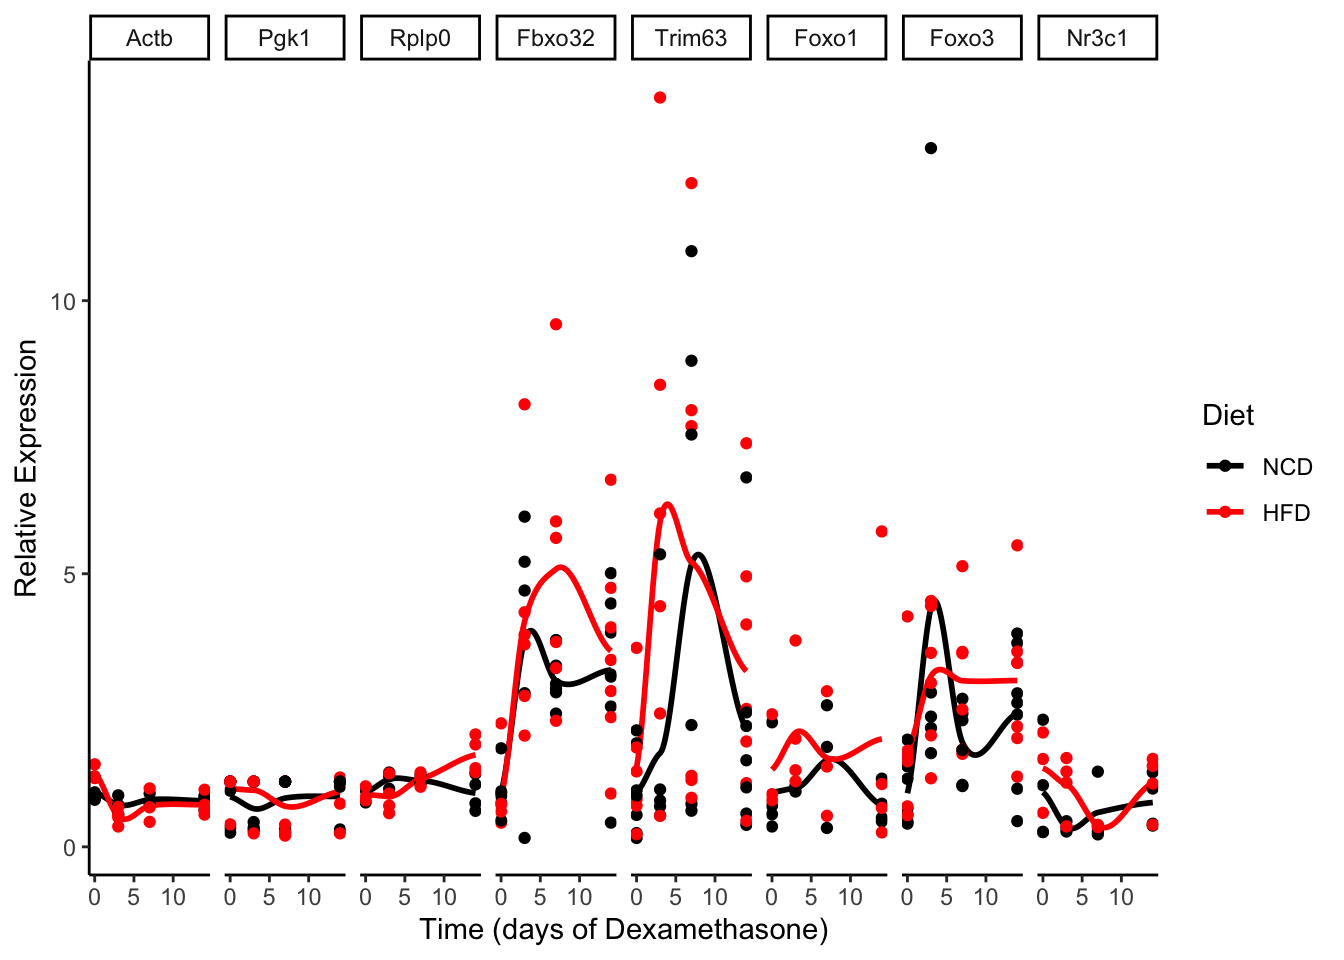
\includegraphics{figures/lineplot-all-points-1.png}

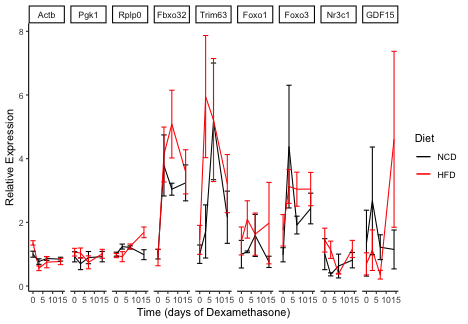
\includegraphics{figures/lineplot-all-1.png}

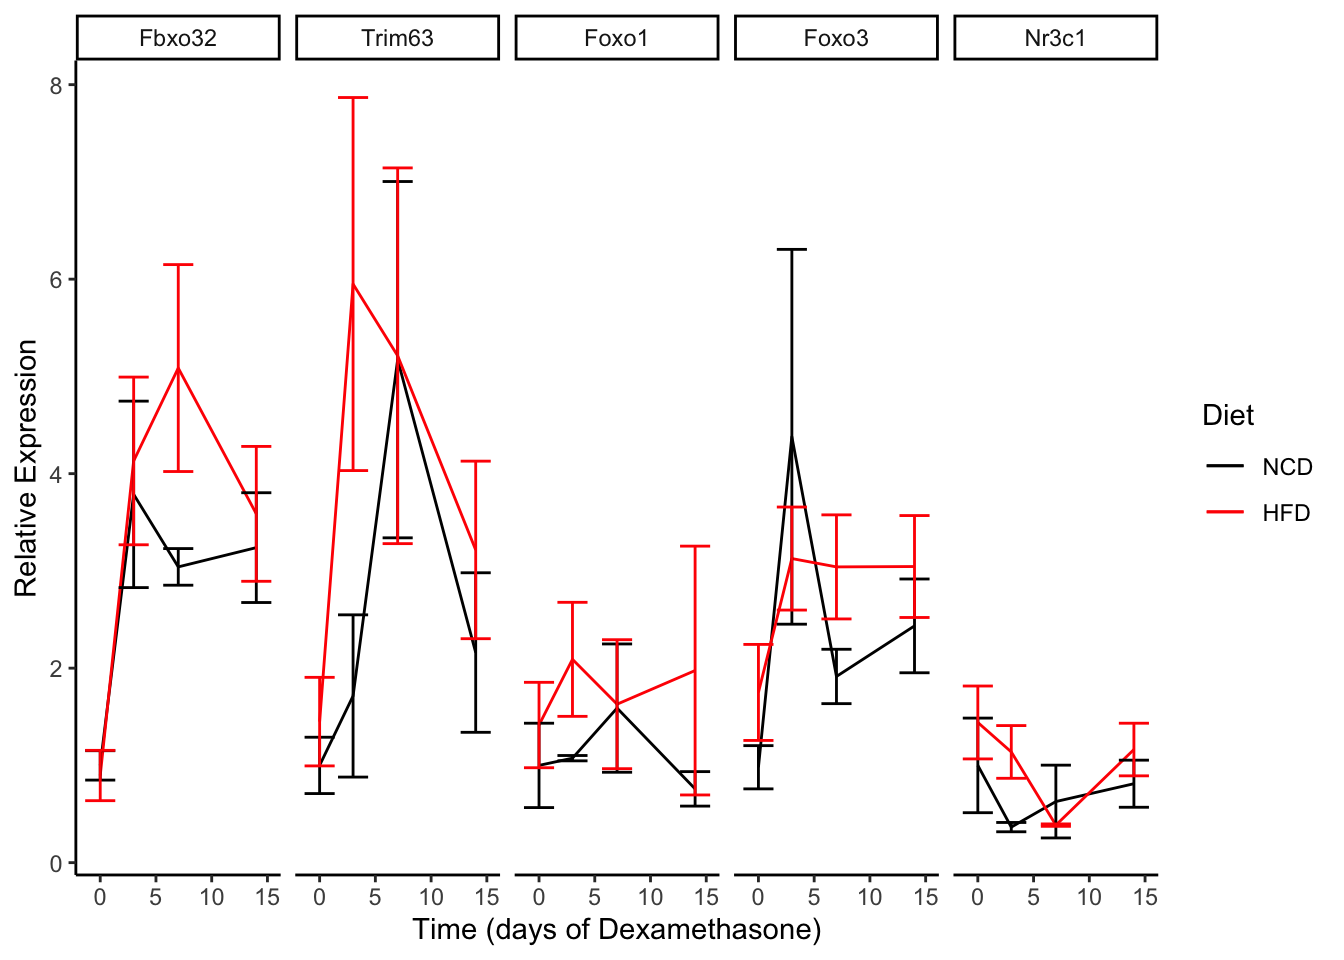
\includegraphics{figures/lineplot-atrogenes-1.png}
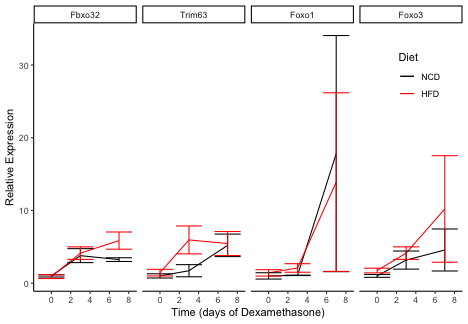
\includegraphics{figures/lineplot-atrogenes-2.png}

\subsection{Statistics}\label{statistics}

\subsubsection{Baseline Effects of Diet}\label{baseline-effects-of-diet}

First tested if there was an effect at baseline for expression of
\emph{Trim63} and \emph{Fbxo32}.

\begin{longtable}[]{@{}lrrrrrr@{}}
\caption{Pairwise statistics for baseline effects of
diet.}\tabularnewline
\toprule
Target Name & HFD.Effect & Shapiro.p & Levene.p & Wilcox.p & Welch.p &
Student.p\tabularnewline
\midrule
\endfirsthead
\toprule
Target Name & HFD.Effect & Shapiro.p & Levene.p & Wilcox.p & Welch.p &
Student.p\tabularnewline
\midrule
\endhead
Fbxo32 & 0.896 & 0.005 & 0.574 & 0.138 & 0.752 & 0.739\tabularnewline
Trim63 & 1.450 & 0.306 & 0.515 & 0.731 & 0.452 & 0.431\tabularnewline
Foxo1 & 1.415 & 0.088 & 0.989 & 0.229 & 0.565 & 0.560\tabularnewline
Foxo3 & 1.784 & 0.075 & 0.440 & 0.181 & 0.226 & 0.187\tabularnewline
Nr3c1 & 1.441 & 0.238 & 0.602 & 0.629 & 0.528 & 0.545\tabularnewline
GDF15 & 0.518 & 0.011 & 0.538 & 0.886 & 0.587 & 0.574\tabularnewline
\bottomrule
\end{longtable}

\subsubsection{Effects of Dexamethasone Over
Time}\label{effects-of-dexamethasone-over-time}

First did pairwise tests at each time point.

\begin{longtable}[]{@{}rlrrrrrrrr@{}}
\caption{Pairwise statistics for effects of diet in dexamethasone
treated animals.}\tabularnewline
\toprule
Time & Target Name & HFD.Effect & Shapiro.p.HFD & Shaprio.p.NCD &
Shapiro.p & Levene.p & Wilcox.p & Welch.p & Student.p\tabularnewline
\midrule
\endfirsthead
\toprule
Time & Target Name & HFD.Effect & Shapiro.p.HFD & Shaprio.p.NCD &
Shapiro.p & Levene.p & Wilcox.p & Welch.p & Student.p\tabularnewline
\midrule
\endhead
0 & Fbxo32 & 0.896 & 0.005 & 0.098 & 0.005 & 0.574 & 0.138 & 0.752 &
0.739\tabularnewline
0 & Trim63 & 1.450 & 0.306 & 0.385 & 0.306 & 0.515 & 0.731 & 0.452 &
0.431\tabularnewline
0 & Foxo1 & 1.415 & 0.119 & 0.088 & 0.088 & 0.989 & 0.229 & 0.565 &
0.560\tabularnewline
0 & Foxo3 & 1.784 & 0.075 & 0.247 & 0.075 & 0.440 & 0.181 & 0.226 &
0.187\tabularnewline
0 & Nr3c1 & 1.441 & 0.630 & 0.238 & 0.238 & 0.602 & 0.629 & 0.528 &
0.545\tabularnewline
3 & Fbxo32 & 1.091 & 0.149 & 0.494 & 0.149 & 0.730 & 0.792 & 0.806 &
0.804\tabularnewline
3 & Trim63 & 3.471 & 0.824 & 0.002 & 0.002 & 0.138 & 0.177 & 0.086 &
0.096\tabularnewline
3 & Foxo1 & 1.946 & 0.213 & 0.370 & 0.213 & 0.203 & 0.057 & 0.181 &
0.203\tabularnewline
3 & Foxo3 & 0.714 & 0.596 & 0.002 & 0.002 & 0.494 & 0.792 & 0.593 &
0.546\tabularnewline
3 & Nr3c1 & 3.116 & 0.466 & 0.678 & 0.466 & 0.241 & 0.114 & 0.062 &
0.063\tabularnewline
7 & Fbxo32 & 1.672 & 0.506 & 0.824 & 0.506 & 0.026 & 0.180 & 0.114 &
0.088\tabularnewline
7 & Trim63 & 1.008 & 0.133 & 0.209 & 0.133 & 0.890 & 0.818 & 0.988 &
0.988\tabularnewline
7 & Foxo1 & 1.025 & 0.772 & 0.650 & 0.650 & 0.986 & 1.000 & 0.968 &
0.968\tabularnewline
7 & Foxo3 & 1.588 & 0.464 & 0.302 & 0.302 & 0.139 & 0.132 & 0.101 &
0.092\tabularnewline
7 & Nr3c1 & 0.614 & 0.434 & 0.078 & 0.078 & 0.359 & 0.700 & 0.584 &
0.553\tabularnewline
14 & Fbxo32 & 1.107 & 0.982 & 0.572 & 0.572 & 0.627 & 0.902 & 0.705 &
0.705\tabularnewline
14 & Trim63 & 1.488 & 0.701 & 0.024 & 0.024 & 0.582 & 0.318 & 0.407 &
0.407\tabularnewline
14 & Foxo1 & 2.604 & 0.046 & 0.391 & 0.046 & 0.319 & 0.886 & 0.413 &
0.383\tabularnewline
14 & Foxo3 & 1.251 & 0.592 & 0.499 & 0.499 & 0.883 & 0.710 & 0.408 &
0.408\tabularnewline
14 & Nr3c1 & 1.433 & 0.376 & 0.273 & 0.273 & 0.910 & 0.343 & 0.371 &
0.370\tabularnewline
\bottomrule
\end{longtable}

Also analysed this with a linear model with diet and time as covariates,
allowing for an interaction. Since time and effect were nonlinear with
respect to each other, used time as a factor, allowing for each time
point to be treated independently.

\begin{longtable}[]{@{}lrrrrr@{}}
\caption{Linear model for effects of time and diet on
Fbxo32}\tabularnewline
\toprule
term & df & sumsq & meansq & statistic & p.value\tabularnewline
\midrule
\endfirsthead
\toprule
term & df & sumsq & meansq & statistic & p.value\tabularnewline
\midrule
\endhead
Diet & 1 & 7.16 & 7.16 & 2.587 & 0.115\tabularnewline
as.factor(Time) & 3 & 78.71 & 26.24 & 9.478 & 0.000\tabularnewline
Diet:as.factor(Time) & 3 & 8.25 & 2.75 & 0.993 & 0.405\tabularnewline
Residuals & 42 & 116.26 & 2.77 & NA & NA\tabularnewline
\bottomrule
\end{longtable}

\begin{longtable}[]{@{}lrrrrr@{}}
\caption{Linear model for effects of time and diet on
Trim63}\tabularnewline
\toprule
term & df & sumsq & meansq & statistic & p.value\tabularnewline
\midrule
\endfirsthead
\toprule
term & df & sumsq & meansq & statistic & p.value\tabularnewline
\midrule
\endhead
Diet & 1 & 26.6 & 26.58 & 2.70 & 0.108\tabularnewline
as.factor(Time) & 3 & 106.5 & 35.50 & 3.60 & 0.021\tabularnewline
Diet:as.factor(Time) & 3 & 30.8 & 10.26 & 1.04 & 0.384\tabularnewline
Residuals & 42 & 413.7 & 9.85 & NA & NA\tabularnewline
\bottomrule
\end{longtable}

\begin{longtable}[]{@{}lrrrrr@{}}
\caption{Linear model for effects of time and diet on
Nr3c1}\tabularnewline
\toprule
term & df & sumsq & meansq & statistic & p.value\tabularnewline
\midrule
\endfirsthead
\toprule
term & df & sumsq & meansq & statistic & p.value\tabularnewline
\midrule
\endhead
Diet & 1 & 0.711 & 0.711 & 1.951 & 0.178\tabularnewline
as.factor(Time) & 3 & 1.766 & 0.589 & 1.616 & 0.217\tabularnewline
Diet:as.factor(Time) & 3 & 0.848 & 0.283 & 0.775 & 0.521\tabularnewline
Residuals & 20 & 7.286 & 0.364 & NA & NA\tabularnewline
\bottomrule
\end{longtable}

\begin{longtable}[]{@{}lrrrrr@{}}
\caption{Linear model for effects of time and diet on
Foxo1}\tabularnewline
\toprule
term & df & sumsq & meansq & statistic & p.value\tabularnewline
\midrule
\endfirsthead
\toprule
term & df & sumsq & meansq & statistic & p.value\tabularnewline
\midrule
\endhead
Diet & 1 & 3.842 & 3.842 & 2.315 & 0.144\tabularnewline
as.factor(Time) & 3 & 0.709 & 0.236 & 0.142 & 0.933\tabularnewline
Diet:as.factor(Time) & 3 & 1.496 & 0.499 & 0.300 & 0.825\tabularnewline
Residuals & 20 & 33.199 & 1.660 & NA & NA\tabularnewline
\bottomrule
\end{longtable}

\begin{longtable}[]{@{}lrrrrr@{}}
\caption{Linear model for effects of time and diet on
Foxo3}\tabularnewline
\toprule
term & df & sumsq & meansq & statistic & p.value\tabularnewline
\midrule
\endfirsthead
\toprule
term & df & sumsq & meansq & statistic & p.value\tabularnewline
\midrule
\endhead
Diet & 1 & 2.66 & 2.66 & 0.796 & 0.377\tabularnewline
as.factor(Time) & 3 & 33.17 & 11.05 & 3.307 & 0.029\tabularnewline
Diet:as.factor(Time) & 3 & 9.61 & 3.20 & 0.959 & 0.421\tabularnewline
Residuals & 42 & 140.39 & 3.34 & NA & NA\tabularnewline
\bottomrule
\end{longtable}

\section{Interpretation}\label{interpretation}

None of these time courses have a significant interaction between time
and diet

\section{Session Information}\label{session-information}

\begin{Shaded}
\begin{Highlighting}[]
\KeywordTok{sessionInfo}\NormalTok{()}
\end{Highlighting}
\end{Shaded}

\begin{verbatim}
## R version 3.5.0 (2018-04-23)
## Platform: x86_64-apple-darwin15.6.0 (64-bit)
## Running under: macOS  10.15.2
## 
## Matrix products: default
## BLAS: /Library/Frameworks/R.framework/Versions/3.5/Resources/lib/libRblas.0.dylib
## LAPACK: /Library/Frameworks/R.framework/Versions/3.5/Resources/lib/libRlapack.dylib
## 
## locale:
## [1] en_US.UTF-8/en_US.UTF-8/en_US.UTF-8/C/en_US.UTF-8/en_US.UTF-8
## 
## attached base packages:
## [1] stats     graphics  grDevices utils     datasets  methods   base     
## 
## other attached packages:
## [1] broom_0.5.2      car_3.0-3        carData_3.0-2    readr_1.3.1     
## [5] ggplot2_3.1.1    dplyr_0.8.3      tidyr_0.8.3.9000 knitr_1.23      
## 
## loaded via a namespace (and not attached):
##  [1] zip_2.0.2         Rcpp_1.0.1        cellranger_1.1.0 
##  [4] pillar_1.4.2      compiler_3.5.0    plyr_1.8.4       
##  [7] highr_0.8         forcats_0.4.0     tools_3.5.0      
## [10] zeallot_0.1.0     digest_0.6.20     lattice_0.20-38  
## [13] nlme_3.1-140      evaluate_0.14     tibble_2.1.3     
## [16] gtable_0.3.0      pkgconfig_2.0.2   rlang_0.4.0      
## [19] openxlsx_4.1.0.1  curl_3.3          yaml_2.2.0       
## [22] haven_2.1.0       xfun_0.7          rio_0.5.16       
## [25] withr_2.1.2       stringr_1.4.0     generics_0.0.2   
## [28] vctrs_0.2.0       hms_0.4.2         grid_3.5.0       
## [31] tidyselect_0.2.5  data.table_1.12.2 glue_1.3.1       
## [34] R6_2.4.0          readxl_1.3.1      foreign_0.8-71   
## [37] rmarkdown_1.13    purrr_0.3.2       reshape2_1.4.3   
## [40] magrittr_1.5      backports_1.1.4   scales_1.0.0     
## [43] htmltools_0.4.0   abind_1.4-5       assertthat_0.2.1 
## [46] colorspace_1.4-1  labeling_0.3      stringi_1.4.3    
## [49] lazyeval_0.2.2    munsell_0.5.0     crayon_1.3.4
\end{verbatim}


\end{document}
